%!TEX program = xelatex
\documentclass[a4paper,10pt,oneside]{article}
\usepackage[UTF8]{ctex}
\usepackage{url}
\usepackage{graphicx}
\usepackage{float}
\usepackage[super, square]{natbib}
\usepackage{booktabs}
\usepackage[margin = 1in]{geometry}
\usepackage{
  color,
  clrscode,
  amssymb,
  ntheorem,
  amsmath,
  listings,
  fontspec,
  xcolor,
  supertabular,
  multirow
}
\usepackage[
  colorlinks,
  linkcolor=bgGray,
  anchorcolor=blue,
  citecolor=black
]{hyperref}
\begin{document}
\lstset{numbers=left,
  basicstyle=\scriptsize\courier,
  numberstyle=\tiny\courier\color{red!89!green!36!blue!36},
  language=C++,
  breaklines=true,
  keywordstyle=\color{blue!70},commentstyle=\color{red!50!green!50!blue!50},
  morekeywords={},
  stringstyle=\color{purple},
  frame=shadowbox,
  rulesepcolor=\color{red!20!green!20!blue!20}
}
\title{一个跑上300MHz的CPU\\[2ex]\begin{large} RISC-V CPU 报告\end{large}}
\author{金乐盛 517030910403}
\maketitle

\section{简介}
此次体系结构大作业要求实现一个基于RISC-V指令集的CPU。

我的GitHub地址:\url{https://github.com/MrTree0-0}

\section{难点}
1. CPU与Memory的带宽为8位,所以对32位数据的操作需要花起码4个周期

2. 如何在上板之后提高运行速度

\section{设计}
实现了标准的五级流水,附带了一些微小的优化:
\paragraph{1.} Data forwarding: 在EX/MEM后把将要写入内存的数据forwarding至ID;在MEM/WB后把将要Write Back的数据forwarding至ID

\paragraph{2.} Static Prediction: 采用Not taken机制,如果后来EX阶段发现错误,将前面流水线寄存器倒空。

\paragraph{3.} Over Clock: 提高CPU时钟频率,最高可达300MHz。(2.8s跑完pi,100MHz情况下约9s)

\section{模拟}
\subsection{主要问题}

\paragraph{1.} 对于时序逻辑和组合逻辑认知不清,以及掌握了一切不正确的语法

解决方法:《夏宇闻-Verilog经典教程》

\paragraph{2.} 调试方法十分低劣

解决方法:机智运用\$dispaly,采用10ns单步调试观察波形图

\paragraph{3.} 改代码及其低效

解决方法:直接将相关模块推倒重写!并且在想清楚模块功能和具体接口之后才落手!

\paragraph{4.} 无法确定自己错误的根源

解决方法:助教给的测试文件往往很长,可以考虑自己写一份十分简短的测试文件。附送一份内存测试代码

\section{上板}
\subsection{主要改动}

\paragraph{1.} 重构与Memory相关部分+重构Register

\paragraph{2.} 查找锁存器

TIPS:使用Synthesis里面的Report Methodology,你可以在Methodology中找到找到所有锁存器latch,鼠标悬停可以找到Source Code
\begin{figure}[H]
  \begin{center}
    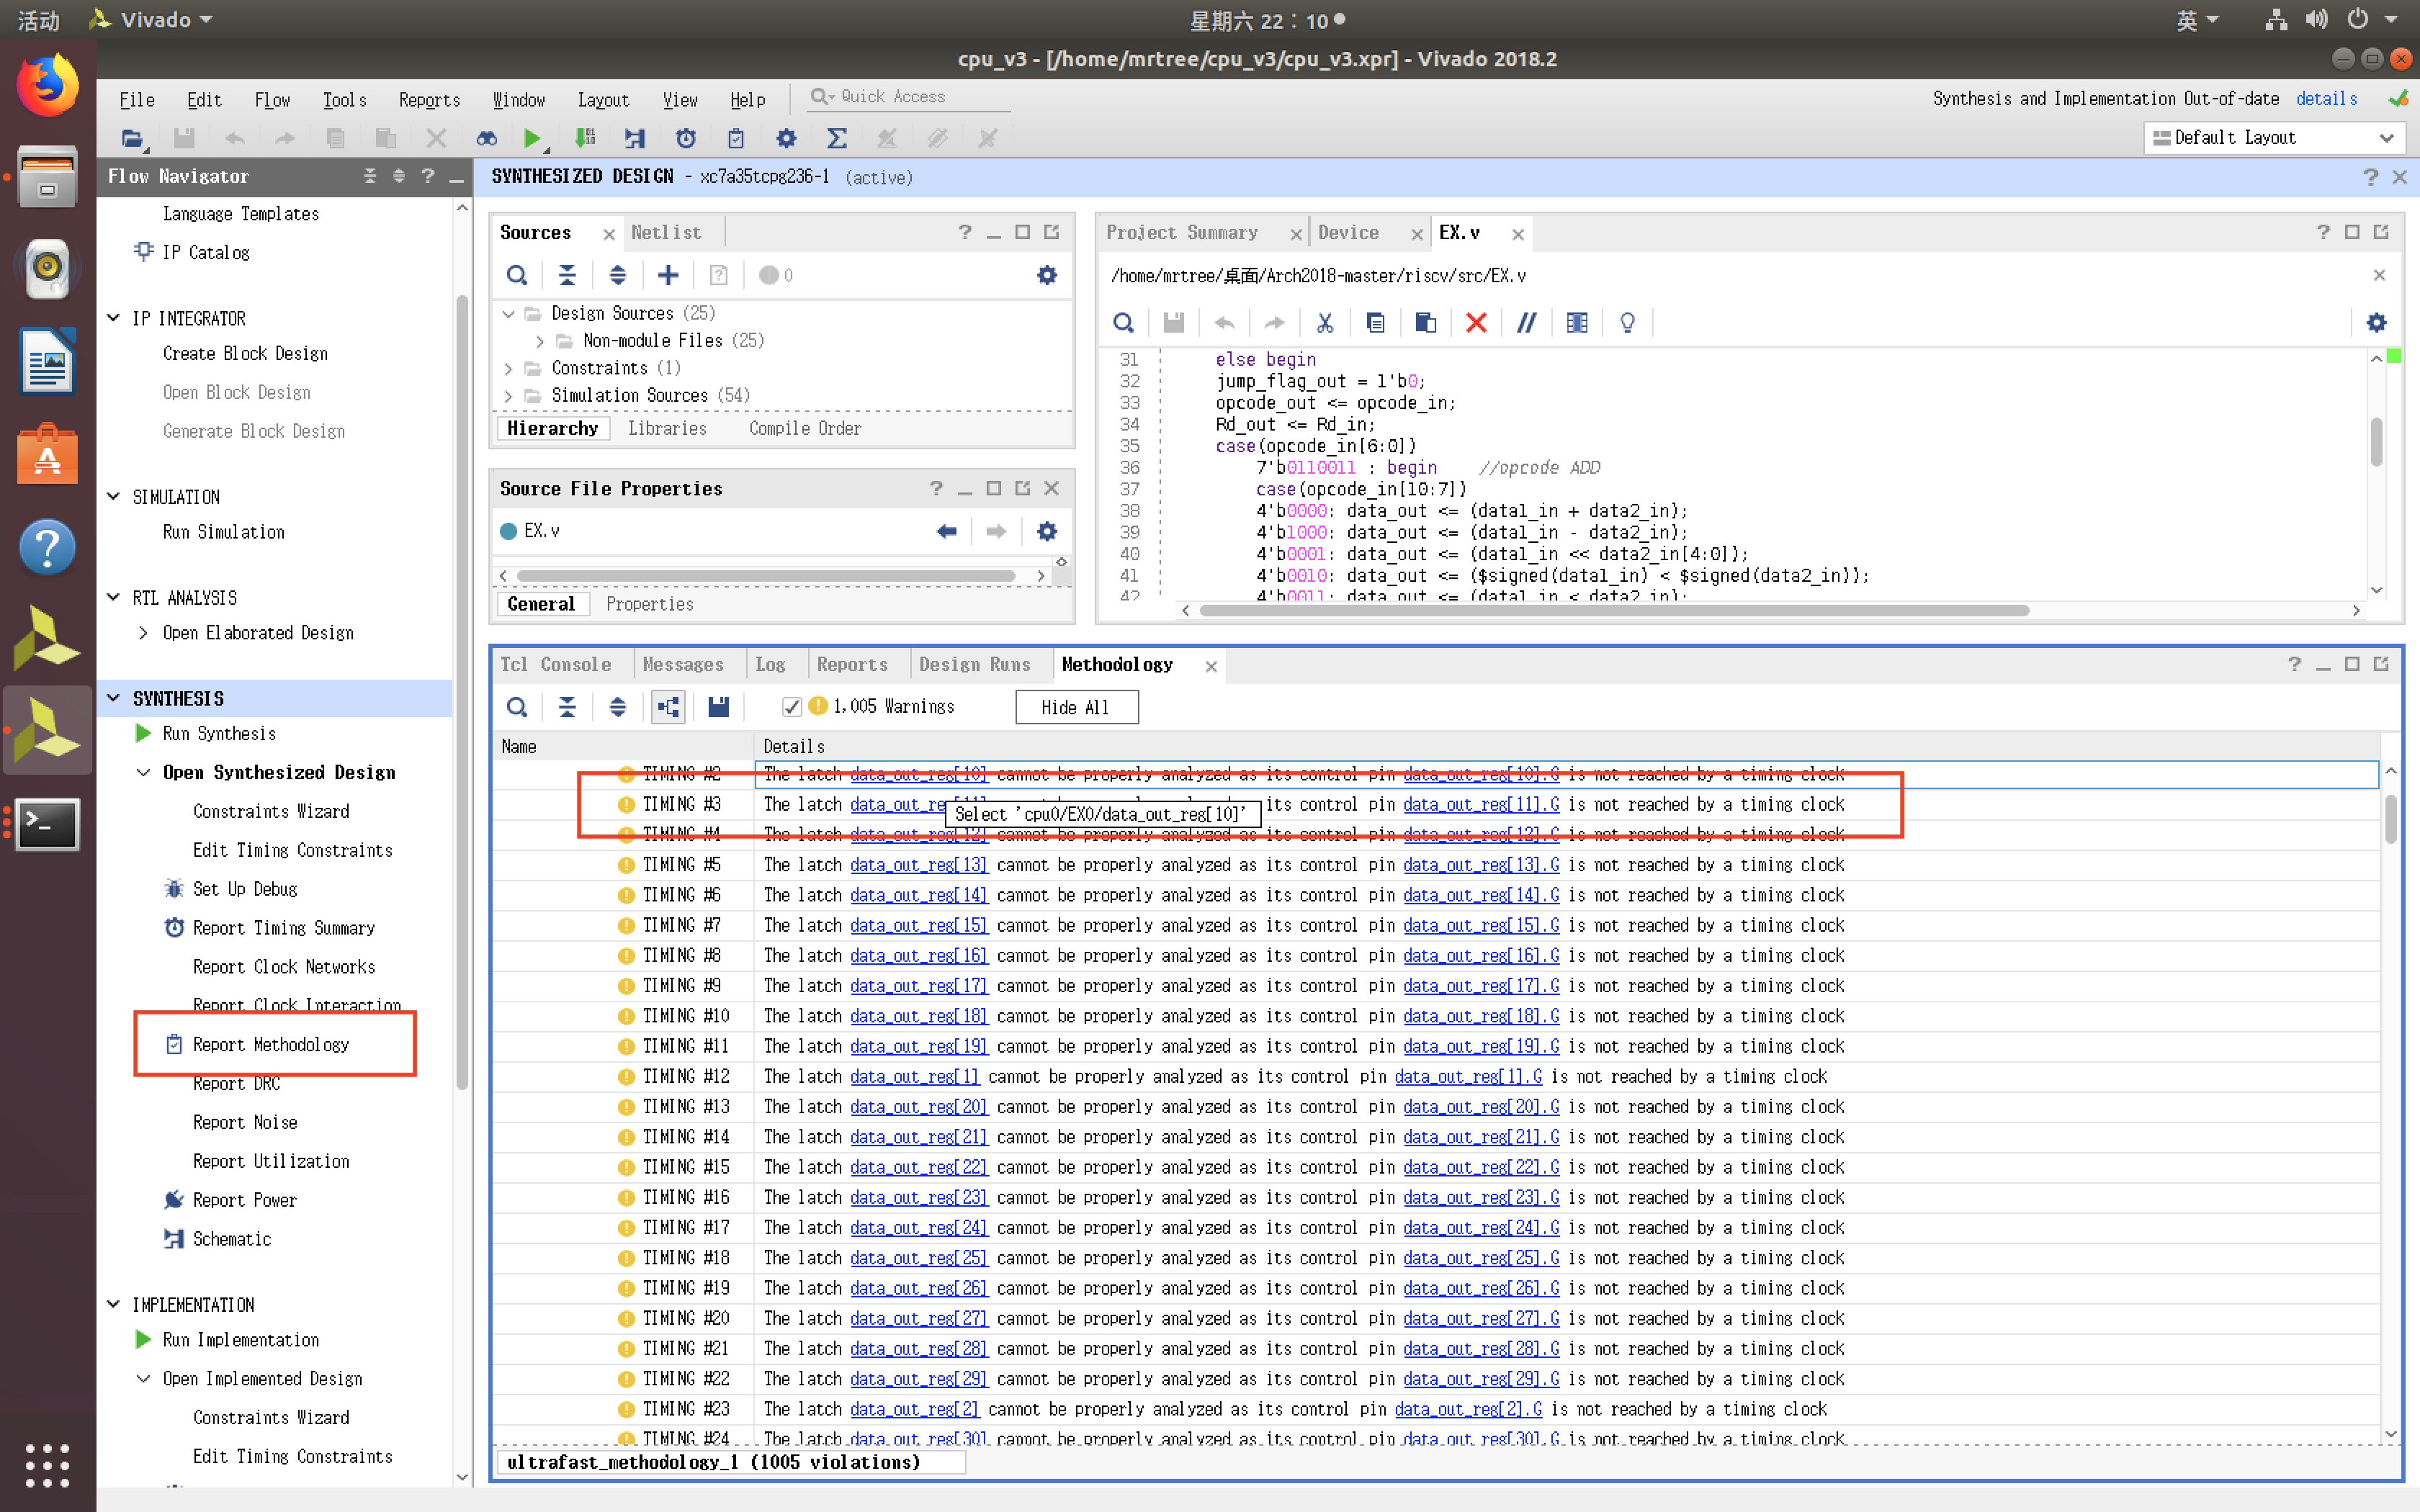
\includegraphics[height=9cm]{latch.png}
  \end{center}
  \caption{注意红框}
\end{figure}

\section{关于调频}
\subsection{最后情况}
300MHz是达到的最高频率,pi的测试结果2.8s,qsort测试能稳定运行。

100MHz情况下,pi的测试结果约为9s。
\begin{table}[H]
\centering
\begin{tabular}{ccc}
\toprule
\multicolumn{1}{c}{频率} & \multicolumn{1}{c}{Old CPU} & \multicolumn{1}{c}{New CPU}\\ 
\midrule
100MHz                  & Yes(MNC $\approx 0.3$)                         & Yes(MNC $\approx 0.3$) \\
150MHz                  & Yes(MNC $\approx 0$)                         & Yes \\
2000MHz                 & No                          & Yes \\
250MHz                  & -                          & Yes \\
300MHz                  & -                          & Yes(MNC $\approx -2.9$) \\
350MHz                  & -                          & No  \\
\bottomrule
%\caption{MNC means Most Negative Slack}
\end{tabular}
\caption{MNC means Most Negative Slack}
\end{table}
\begin{figure}[H]
  \begin{center}
    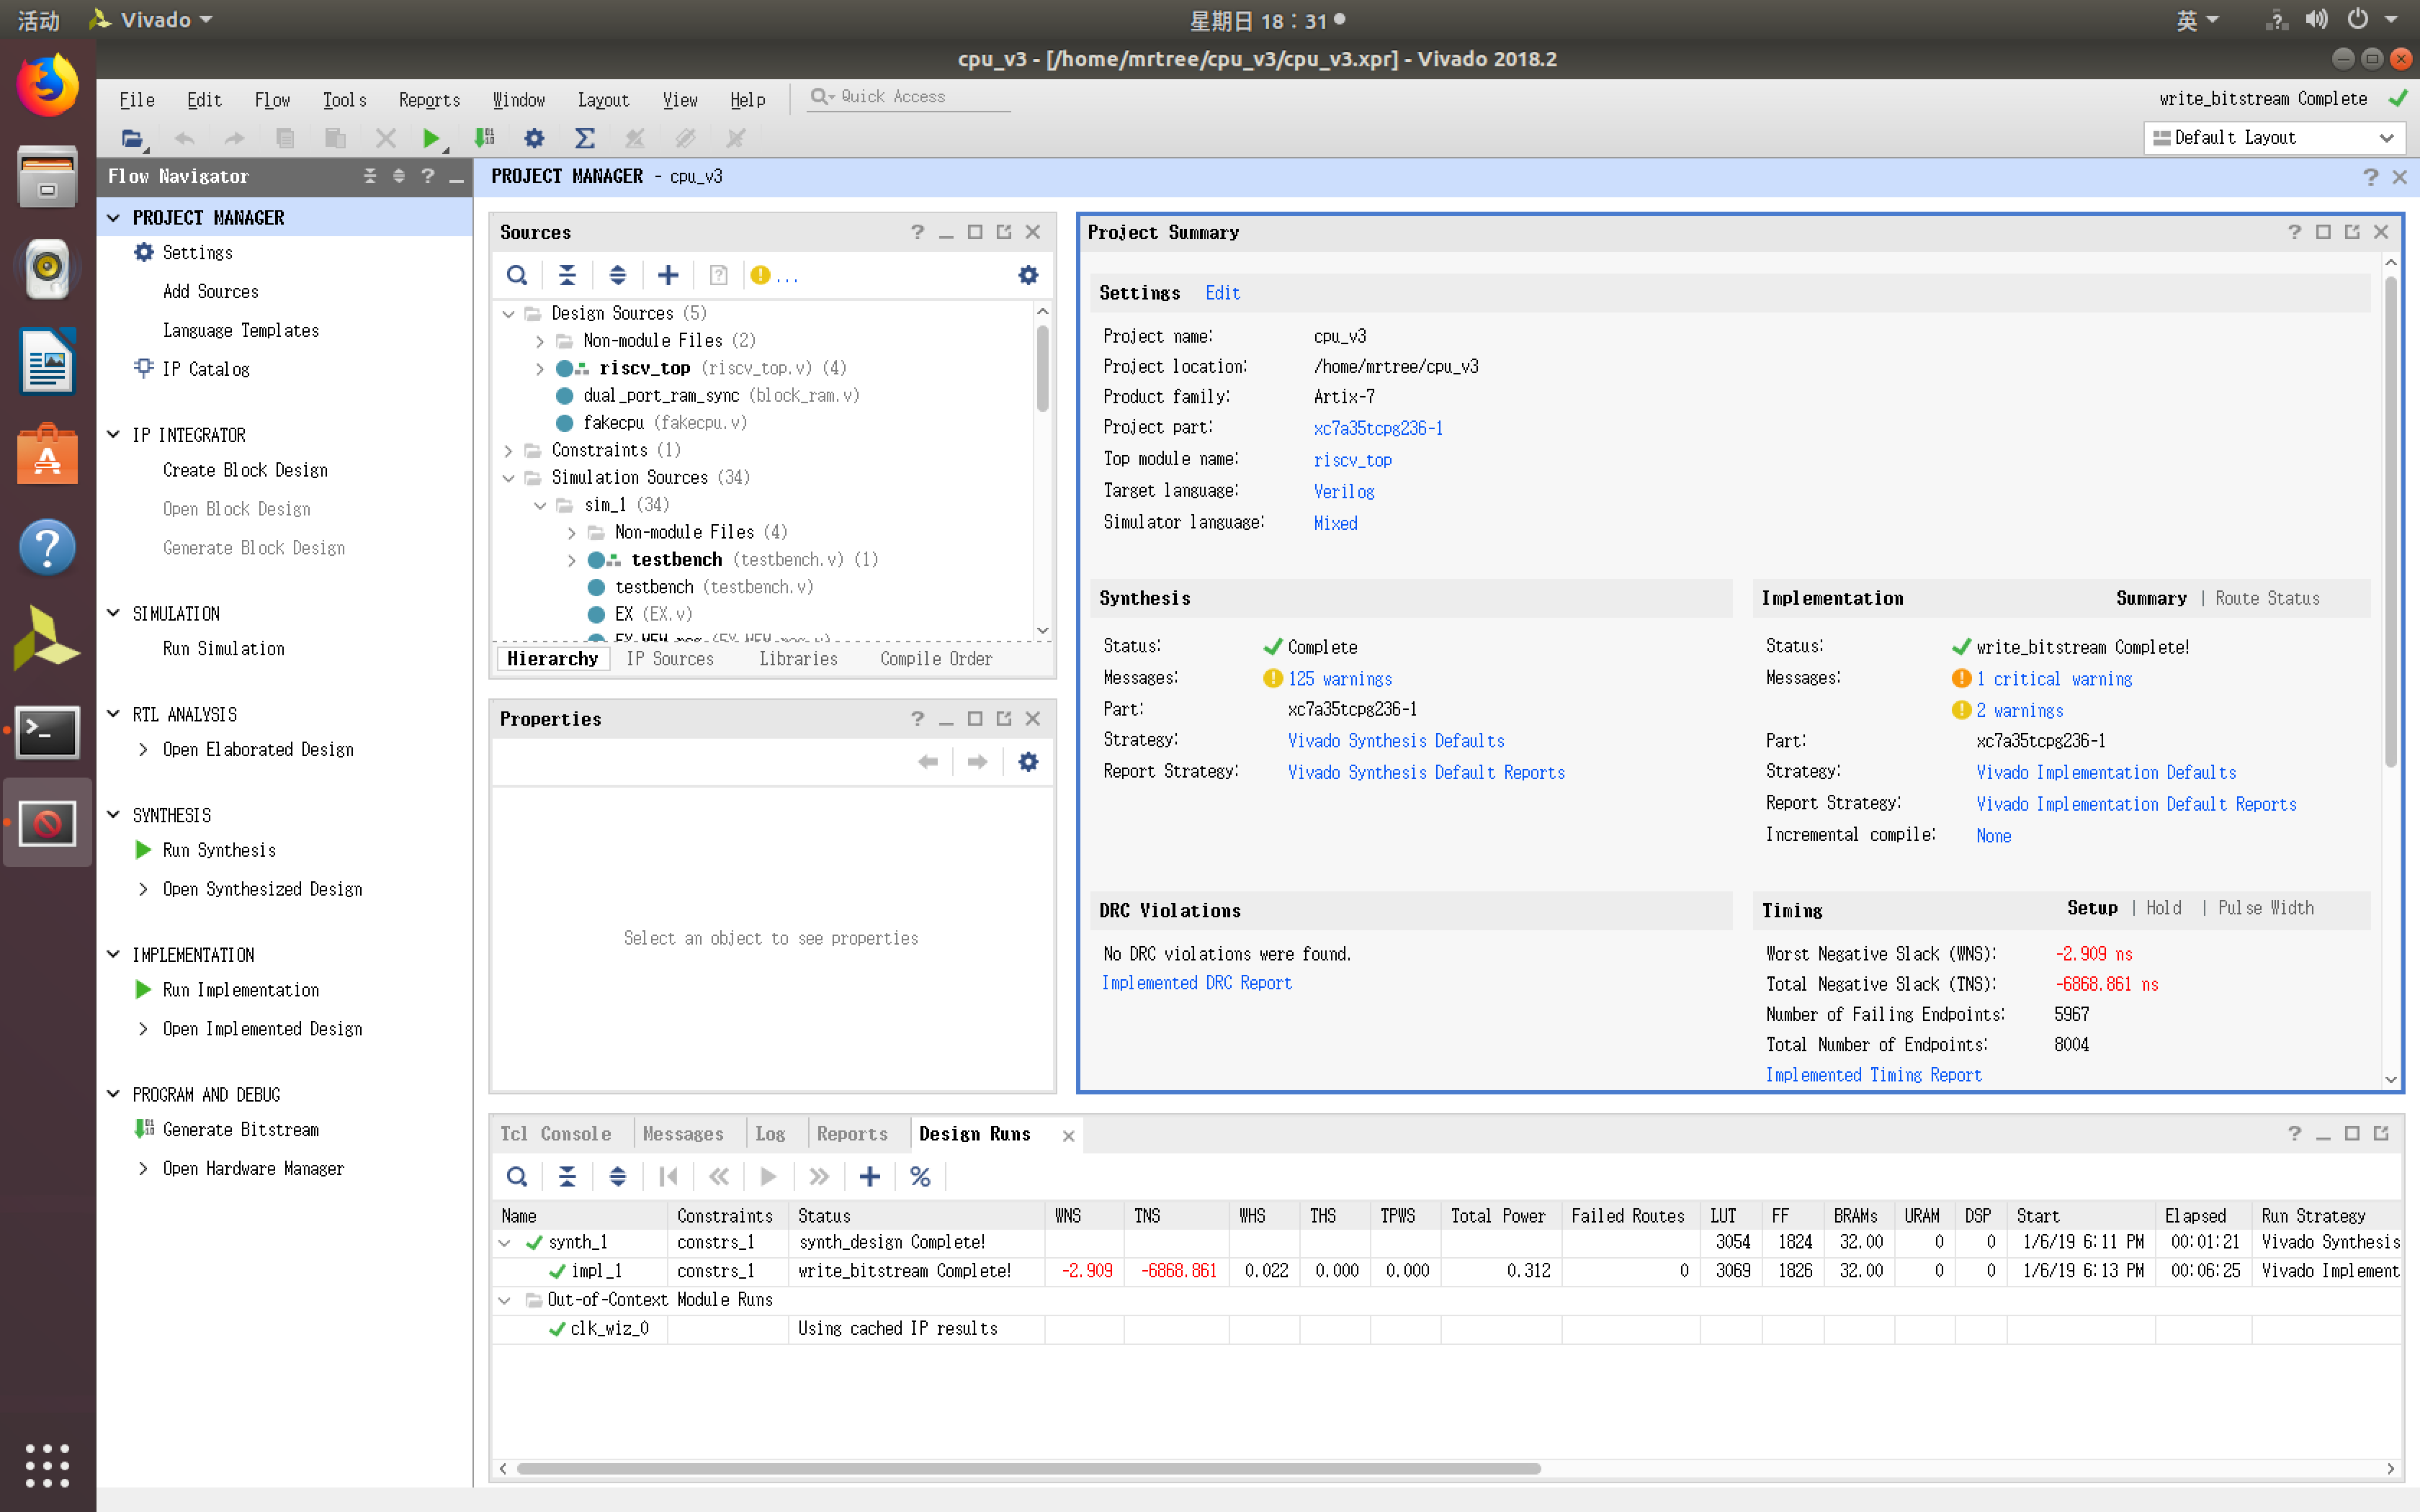
\includegraphics[height=9cm]{300MHz-MNC.png}
  \end{center}
  \caption{300MHZ -2.9MNC}
\end{figure}

\subsection{短板效应} 整个CPU中限制频率的是耗时最长的模块。 诸如像ID、EX、WB这些模块都是组合逻辑,always@* 的操作在布线的时候或多或少会被简化,想当于一堆assign连线,个人认为优化空间不大。 有时序逻辑的地方应该是被简化的重点,所以就开始重构。

\subsection{优化过程} 在流水线寄存器方面没什么优化,因为本来就写成了DQ锁存器的形式。 然后重点攻克Memory方面,重点是完全采用时序逻辑,完全采用非阻塞赋值,在数据读取或者写入完成后hold一个周期(这个可能可以淡化一部分电路延迟的弊端)。

\section{总结与思考}
\subsection{用最简单的想法写最简单的代码做最简单的事!} 

\subsection{与Memory的斗争} 
\paragraph{CPU\_V0}在Memory方面,本人不惜代价去抢拍,采用各种奇怪的写法,其中多数是时序+组合混用。结果是几乎把能抢到拍都抢了,就是数据一旦读取完成,在busy信号拉低的同时,把数据取走。这种混乱的抢拍在模拟的时候波形图无比完美,但是一旦在FPGA上运行时,一点小小的延迟就会让程序乱跑。

\paragraph{CPU\_V1}就如上面所说本人开始放弃抢拍的操作了,甚至在mem\_ctrl把数据读完以后,过一个周期CPU才会去读。这种简单的写法不仅大大简化了电路,并且保证了数据的稳定性。

\section{感谢}
感谢梁老师、助教和各位同学们的帮助。特别感谢苏起冬同学对本人的指导——“小而快”。特别感谢陈林淇同学对本人上板调试的帮助。
\begin{thebibliography}{9}
  \bibitem{lsl}
    雷思磊.
    \emph{自己动手写CPU},
    电子工业出版社, 2014.
  \bibitem{lsl}
    夏宇闻.
    \emph{Verilog经典教程}
  \bibitem{caqa} 
  John L. Hennessy, David A. Patterson, et al.
  \emph{Computer Architecture: A Quantitative Approach},
  Fifth Edition, 2012.
  \bibitem{ppt}
  David A. Patterson.
  PPT of \emph{CS252 Graduate Computer Architecture},
  2001.
  
\end{thebibliography}
\end{document}